%Introdução

\chapter{Introdução}

Este trabalho acadêmico demonstra a aplicação da Lógica Paraconsistente Anotada (LPA), em jogos do gênero \textit{Tranding Card Games} (Jogos de Cartas Colecionáveis – TCG), através da criação de uma biblioteca de \dfrac{Tomada}{den} de Decisão que implementa a Lógica Paraconsistente Anotada Evidencial (LPA E$\tau$), além disso será criado um jogo de cartas que utiliza a biblioteca para demonstrar as suas funcionalidades.

Com parte do senso comum, as pessoas acreditam que os jogos têm como única finalidade entreter ignorando as diversas opções que um jogo eletrônico pode trazer para auxiliar o desenvolvimento humano, de modo que a utilização dos jogos de forma educacional ou para resolver problemas usando raciocínio lógico pode trazer benefícios à saúde \cite{fabio-luis-lpa}.

A LPA é uma lógica não clássica que admite contradições e incertezas, é uma boa solução para fazer tratamento de situações reais, no qual a Lógica Clássica, por ser binária, se mostra ineficaz ou impossibilitada de ser aplicada \cite{metodos-lpa-2006}. Assim possibilita as mais variadas aplicações em áreas tais como computação, robótica, tráfego aéreo e de trens, distribuição de energia em grandes usinas, programação, redes neurais, pesquisa operacional entre outras \cite{tomda-decisao-lpa-2011}.

Uma biblioteca é uma coleção de subprogramas ou um programa que facilita o desenvolvimento de sistemas, no núcleo da biblioteca desenvolvida será utilizado a
LPA. Dessa forma a biblioteca implementada no jogo será responsável por tomar as decisões dos resultados de batalha, sendo o intuito de criar um software que pode ser reutilizável por outros, iniciando um estudo da aplicação da LPA em jogos TGC.

Será explicado como a biblioteca foi desenvolvida e implementada no jogo, juntamente com a sua documentação para utilização. Também será relatado como o
jogo foi desenvolvido, quais ferramentas e metodologias foram utilizadas e quais resultados que foram obtidos em vantagem com a utilização da LPA.

Este documento está estruturado nos seguintes tópicos, \textit{1 - Introdução} apresenta o projeto, os objetivos e as justificativas. No capítulo \textit{2 - Referência Teórica} é
exposta a base conceitual do projeto. Na seção seguinte \textit{3 - Materiais e Métodos} é retratada a metodologia utilizada para desenvolvimento da prototipagem além das ferramentas utilizadas no processo. [EM CONSTRUÇÃO]

Terminada a descrição da estrutura do trabalho, prossegue para \textit{capítulo 2 - Referência Teórica}.

\section{Justificativa}

No desenvolvimento de jogos de cartas, é encontrado diversas bibliotecas disponibilizado na \textit{Unity Asset Store}, com uso de lógica clássica, que uma proposição é classificada como verdadeira ou falsa. Não há qualquer outra possível alternativa, ou algo é Verdadeiro ou exclusivamente Falso \cite{aspectos-lpa-2013}.

A lógica paraconsistente introduz duas novas categorias além do Verdadeiro e do Falso. Podemos ter proposições classificadas como Verdadeiras, Falsas, Inconsistentes ou Paracompletas. Para uma proposição ser classificada com Inconsistente tem haver uma evidência sugere que ela seja Verdadeira e outra evidência sugere que ela é Falsa, Agora quando não tem evidência Verdadeira nem tampouco que ela seja Falsa a proposição é classificada como Paracompleta \cite{aspectos-lpa-2013}.

Sendo que a Logica Paraconsistente é utilizado em outras áreas e não é utilizado especificamente em jogos e cartas. Portanto a proposta do projeto é desenvolver uma biblioteca aplicando Tomada de Decisão com Lógica Paraconsistente ao invés do Logica clássica, para auxiliar no processo decisório de uma forma ágil e eficiente.


\section{Validação Empírica}

A LPA é uma lógica não clássica que aceita contradições. A partir disso criar um cenário de jogo de cartas para demonstrar o uso da
paraconsistente. Para exemplificar, foram criadas quatro cartas com atributos de força e velocidade com valores favoráveis e desfavoráveis de acordo com arma e idade conforme a tabela \ref{tab:cartas}.

\begin{table}[htb]
	\centering
	\caption{Visualização das Cartas}
	\label{tab:cartas}
	\begin{tabular}{|l|l|l|l|l|l|}
		\hline
		\textbf{Carta}              & \textbf{Atributos}  & \textbf{Favorável} & \textbf{Desfavorável} & \textbf{Detalhes} & \textbf{Valor} \\ \hline
		\multirow{2}{*}{Arqueiro}   & \textit{Força}      & 20                 & 10                    & \textit{Arma}     & Arco e Flecha  \\ \cline{2-6} 
		& \textit{Velocidade} & 70                 & 35                    & \textit{Idade}    & 25             \\ \hline
		\multirow{2}{*}{Espadachim} & \textit{Força}      & 55                 & 20                    & \textit{Arma}     & Espada         \\ \cline{2-6} 
		& \textit{Velocidade} & 40                 & 20                    & \textit{Idade}    & 19             \\ \hline
		\multirow{2}{*}{Lanceiro}   & \textit{Força}      & 50                 & 10                    & \textit{Arma}     & Lança          \\ \cline{2-6} 
		& \textit{Velocidade} & 68                 & 35                    & \textit{Idade}    & 30             \\ \hline
		\multirow{2}{*}{Bárbaro}    & \textit{Força}      & 70                 & 50                    & \textit{Arma}     & Martelo        \\ \cline{2-6} 
		& \textit{Velocidade} & 60                 & 80                    & \textit{Idade}    & 40             \\ \hline
	\end{tabular}
	\fonte{Produzido pelos autores.}
\end{table}

O primeiro passo é realizar o processo de maximização, a partir do qual se obtém os maiores valores das evidências favoráveis e os menores das evidências
desfavoráveis, entre as cartas \textit{Arqueiro} e \textit{Espadachim}, repetindo o processo em relação às cartas \textit{Lanceiro} e \textit{Bárbaro}. Na sequência, realiza-se o processo de minimização, o qual consiste na obtenção dos menores valores das evidências favoráveis e dos maiores valores das evidências desfavoráveis, as quais foram maximizadas anteriormente.
Após realizar o processos de maximização e minimização nos dois atributos das cartas, obteve-se os seguintes valores:

\begin{figure}[htb]
	\caption{
		\label{fig:forca} 
		Valores
	}
	\begin{center}
		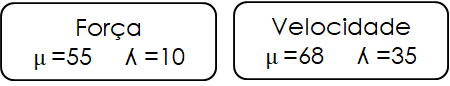
\includegraphics[scale=0.5]{imagens/valores.png}
	\end{center}
	\legend{Fonte: Produzido pelos autores.}

\end{figure}

Após a realização da maximização entre esses valores chegou-se ao seguinte resultado:

\begin{figure}[htb]
	\caption{
		\label{flg:max}
		Maximização
	}
	\begin{center}
		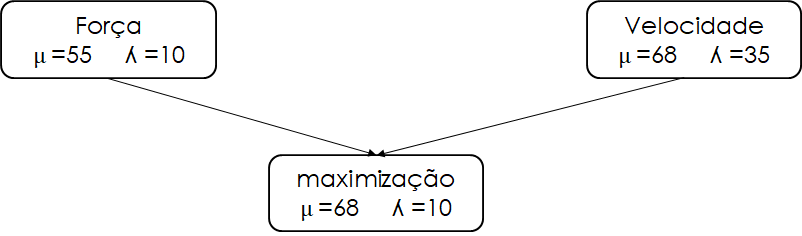
\includegraphics[scale=0.5]{imagens/max.png}
	\end{center}
	\legend{Fonte: Produzido pelos autores.}	
\end{figure}

Aplicando o grau de certeza e incerteza sobre esses valores a saída foi o seguinte estado lógico:

\begin{equation*}
	\begin{array}{cc}
	Gi = 0.68 + 0.1 -1 = -0.22 \\
	Gc = 0.68 - 0.1 = 0.58
	\end{array}
\end{equation*}

Através do estado lógico foi produzido o parecer analítico com uma tabela pré definida cujo resultado refere-se a porcentagem que as 4 cartas conseguem tirar de vida do adversário.

\newpage

\begin{table}[htb]
	\centering
	\caption{Relação entre o status e parecer analítico}
	\label{tab:analitica}
	\begin{tabular}{cc}
		\hline
		\multicolumn{1}{|c|}{\textbf{Status}} 	& \multicolumn{1}{c|}{\textbf{Parecer Analítico}} \\ \hline
		$V$               						& 100\%                      \\
		$F$               						& 0\%                        \\
		$T$               						& 0\%                        \\
		$\bot$									& 0\%                        \\
		$T \rightarrow V$             			& 20\%                       \\
		$T \rightarrow F$            			& 10\%                       \\
		$V \rightarrow \bot$            		& 16\%                       \\
		$F \rightarrow \bot$            		& 8\%                        \\
		$Qv \rightarrow T$            			& 50\%                       \\
		$Qv \rightarrow \bot$           		& 40\%                       \\
		$Qf \rightarrow T$            			& 6\%                        \\
		$Qf \rightarrow \bot$           		& 2\%                       
	\end{tabular}
	\fonte{Produzido pelos autores.}
\end{table}

O status obtido na maximização foi $T \rightarrow F$, conforme a tabela \ref{tab:analitica} a porcentagem seria de 10\%, com essa validação possuí a lógica que será aplicada para Tomada de Decisão no jogo, assim iniciar a criação da dinâmica do jogo.

\section{Objetivos}

O objetivo geral é desenvolver uma biblioteca de Tomada de Decisão que utilize a LPA com foco em jogos TCG com objetivo de, protótipo final, isso é, biblioteca com manual de utilização e jogo de demostração, com o intuito de ser utilizada por outros desenvolvedores de jogos de cartas


\section{Objetivos Específicos}
	\begin{itemize}
		\item Criar o modelo de paraconsistente a ser utilizado.
		\item Criar a biblioteca aplicando a LPA E$\tau$.
		\item Criar uma versão da biblioteca com valores fixo para uma implementação no jogo sem muitos problemas.
		\item Desenvolver uma segunda versão da biblioteca, permitindo que ela seja genérica o suficiente para atender diferentes regras de negócio em jogos TCG.
		\item Desenvolvimento da biblioteca.
		\item Construir um manual de utilização e documentação da biblioteca.
		\item Criar um jogo do gênero TCG que demonstre as funcionalidades da biblioteca.
		\item Gerar \textit{Asset} e disponibilizar na plataforma \textit{Unity Asset Store}.
		\item Criar a presente documentação descrevendo os materiais, métodos e referências utilizadas para a construção do projeto.
	\end{itemize}


